
\section{Evaluation}
\subsection{Time series forecasting of periodic functions}
\label{sec:sine}
In the first part of the analysis, we analyze the capability of different neural
network architectures to perform time series prediction on the periodic sinus
function. This task can be considered simple, because the different parts of the
sine wave occur multiple times in the data.
It is therefore interesting how
robust the network architectures are with regard to different kinds of noise.

In this problem, we apply a large grid search over several parameters given in
Table~\ref{tab:gridparameters}. All models are trained using the \emph{Adam}
optimizer and $10$ time sequence entries are used to predict $1$ directly
consecutive point. These assumptions are made in order to keep the grid search
feasible. For training, testing and validation, a range from $0$ to $6 \pi$ is
used. The data is split equally between the datasets, the first third used as 
the training and the second third used as the validation set.
Expressed more formally,
we provide information about the last 10 time sequence points
to the network and want to predict the next point, as given in
Equation~\ref{equ:sine}. That is, we want to estimate $x(t)$ with a function
$F(x(t), x(t-1), \cdots, x(t-9))$ that is computed using a neural network.

\begin{equation}
    \hat{x} (t + 1) \approx F(x(t), x(t-1), \cdots, x(t-9))
    \label{equ:sine}
\end{equation}


\begin{table}
    \centering
    \begin{tabular}{l|c}
        Parameter                   & Values                    \\
        \hline
        Number of hidden nodes      & [5, 10, 20]               \\
        std ($\sigma$) of noise     & [0, 0.01, 0.1]            \\
        Noise type                  & ["iid", "Wiener process"] \\
        Learning rate               & [0.001, 0.01, 0.1]        \\
        Epochs of training          & [10, 100, 500]            \\
        Neural network architecture & ["MLP", "LSTM", "CNN"]    \\
    \end{tabular}
    \caption{Parameter combinations used for the grid search. Each possible value
        of each parameter is combined with each possible value of each other
        parameter. Note that the \emph{CNN}s are evaluated with 1, 2, or 3 hidden
        layers of with 8 filters instead.}
    \label{tab:gridparameters}
\end{table}
%todo: mg adam justification

As we expected from our literature review, the \emph{LSTM} yielded lowest error
on the noise free time series data as seen in Table~\ref{tab:noisefree_result}.
After investigating the high error for the \emph{CNN} architecture, we discover
that this architecture needs a lower training rate than the \emph{LSTM}
architecture to yield good results -- the learning rate of $0.1$ is too high
and ruins the results as seen in Table~\ref{tab:cnn_training}.

\begin{table}
    \centering
    \begin{tabular}{l|c}
        Architecture & Average MSE \\
        \hline
        MLP          & 0.00285     \\
        LSTM         & 0.00066     \\
        CNN          & 0.07583     \\
    \end{tabular}
    \caption{Average MSE over all applied neural networks aggregated by
        the neural network architecture type.}
    \label{tab:noisefree_result}
\end{table}

\begin{table}
    \centering
    \begin{tabular}{l|c|c}
        Learning rate & Average MSE (CNN) & Average MSE (LSTM)       \\
        \hline
        0.1           & 0.227052          & 5.391024 $\cdot 10^{-5}$ \\
        0.01          & 0.000155          & 8.129514 $\cdot 10^{-5}$ \\
        0.001         & 0.000159          & 0.000276                 \\
    \end{tabular}
    \caption{Comparison of the average MSE when training \emph{CNN} and
        \emph{LSTM} architectures. We see that the \emph{LSTM} can be trained
        using higher learning rates.}
    \label{tab:cnn_training}
\end{table}

Next we investigate the influence of the type of noise
and the standard deviation of the noise on the results 
based on our grid search. The average error is
strongly impacted as seen in Table~\ref{tab:wiener_iid}. We see that
a higher $\sigma$ increases the test error, as expected. But it seems that the 
neural networks are less capable of filtering noise from a Wiener process, and 
for a high $\sigma$ of this type of noise completely lose the ability to 
approximate the underlying sinus function on the first look. A further analysis
of the used networks architectures shows that this is merely caused by inluding 
\emph{CNN}s trained with learning rate $0.1$. After excluding them, the test 
error goes down to a high but reasonable value.

\begin{table}
    \centering
    \begin{tabular}{l|ccc}
        Type of noise & MSE & MSE ($\sigma=0.01$) & MSE($\sigma=0.1)$) \\
        \hline
        $i.i.d$ noise &   0.015 & 0.008  &  0.022 \\
        Wiener process & 24.153 & 0.0524 & 48.254 (1.322) \\
    \end{tabular}
    \caption{Average MSE aggregated by the type of noise and the noise
        standard deviation.}
    \label{tab:wiener_iid}
\end{table}

In Figure~\ref{fig:sinenoisefree}, we see the best neural networks found using 
the large grid search for a noise free time series. The approximation is 
remarkably accurate and no deviation can be found. If we add different kinds of 
noise, the grid search is still able to find suitable architectures, 
as seen in Figure~\ref{fig:sineresult}. In Figure~\ref{fig:histogram}
we demonstrate that only a few outliers caused the average error 
for Wiener process noise with high $\sigma$ to increase so strongly.

After 
investigating the architectures of the best neural networks in 
Table~\ref{tab:architectures}, we conclude that \emph{LSTM} networks are best 
suitable to situations in which noise with high variance occurs. But also a 
classical \emph{MLP} architecture performed best in presence of high Wiener
noise, while for a small amount
of Wiener noise, the \emph{CNN} architecture is advantageous. From the 
grid search, we conclude furthermore that the default parameters in the 
optimization algorithms can be improved in various cases. The longest training
is not always delivering the best results, which indicates the importance of 
the Early Stopping technique. Using the grid search on a various number of
parameters, it was possible to find a suitable architecture for each of the
considered situations.

\begin{figure}
    \centering
    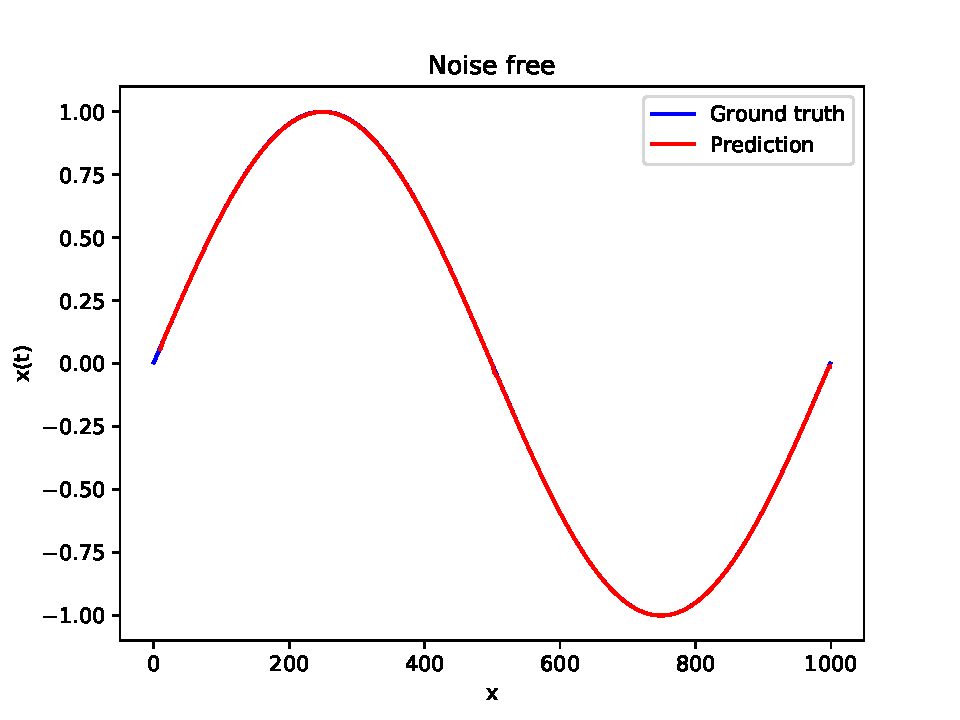
\includegraphics[width=0.6\textwidth]{figures/Noise_free.pdf}
    \caption{Demonstration of grid search results. For the noise free case,
    a nearly perfect approximation is achieved.}
    \label{fig:sinenoisefree}
\end{figure}

\begin{figure}
    \centering
    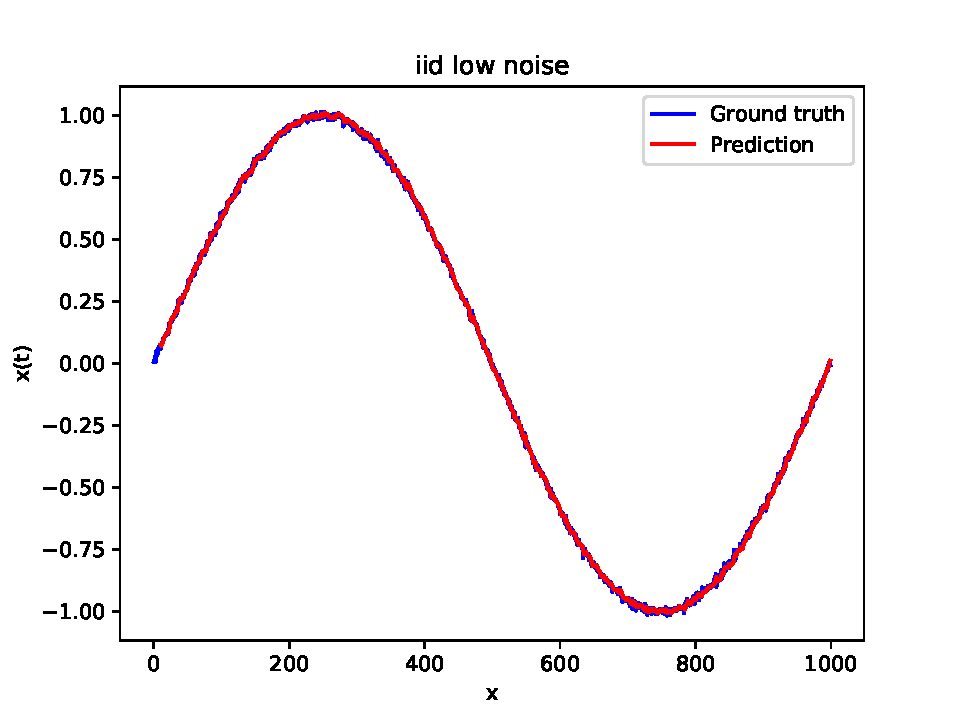
\includegraphics[width=0.45\textwidth]{figures/iid_low_noise.pdf}
    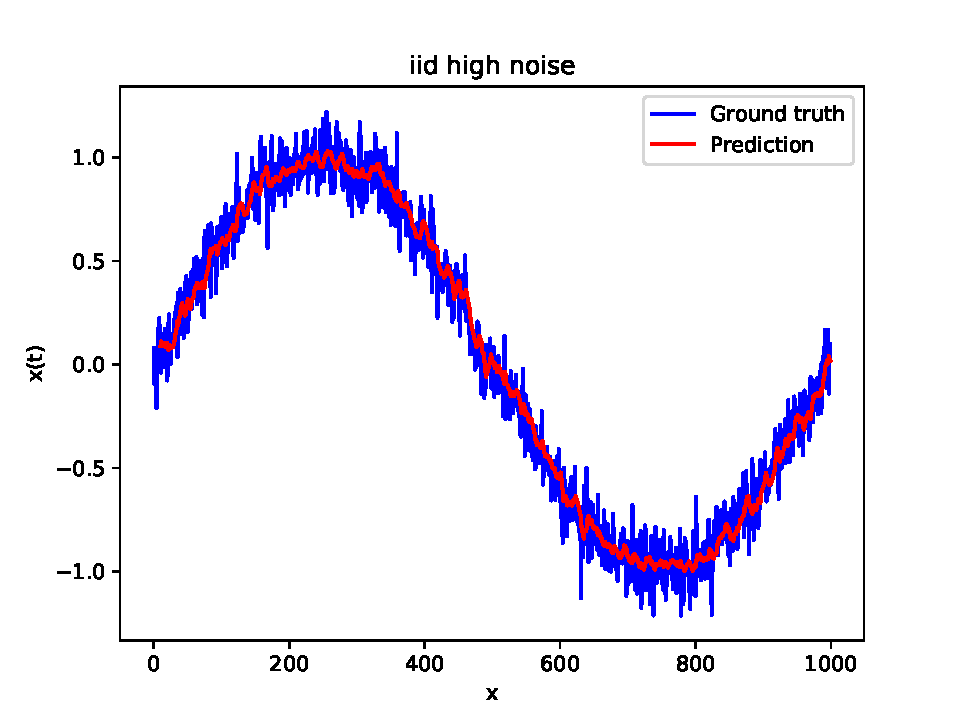
\includegraphics[width=0.45\textwidth]{figures/iid_high_noise.pdf}
    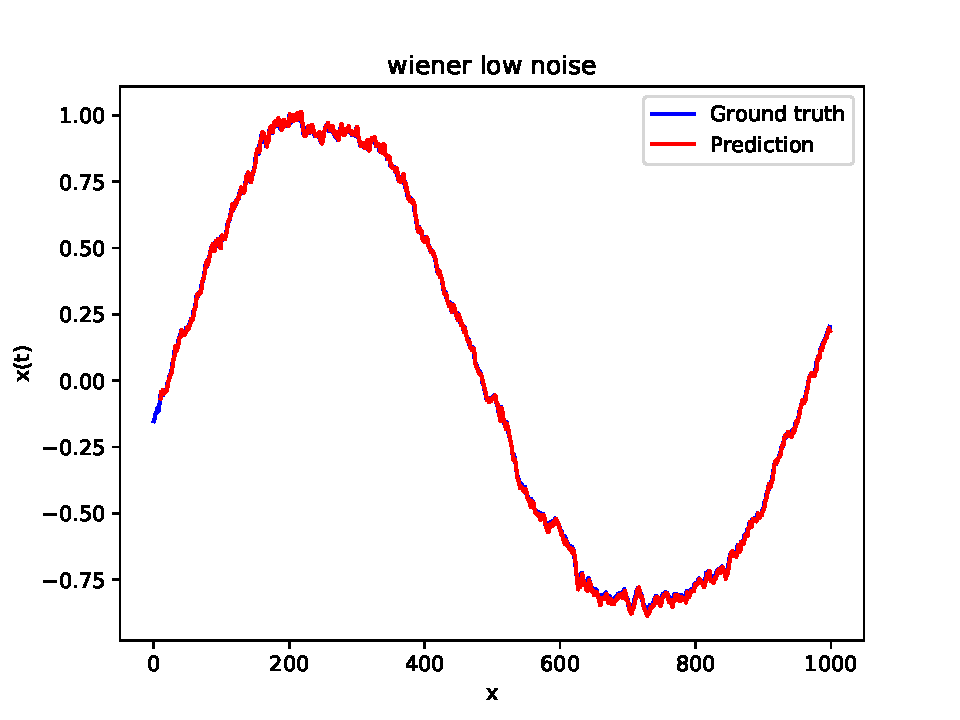
\includegraphics[width=0.45\textwidth]{figures/wiener_low_noise.pdf}
    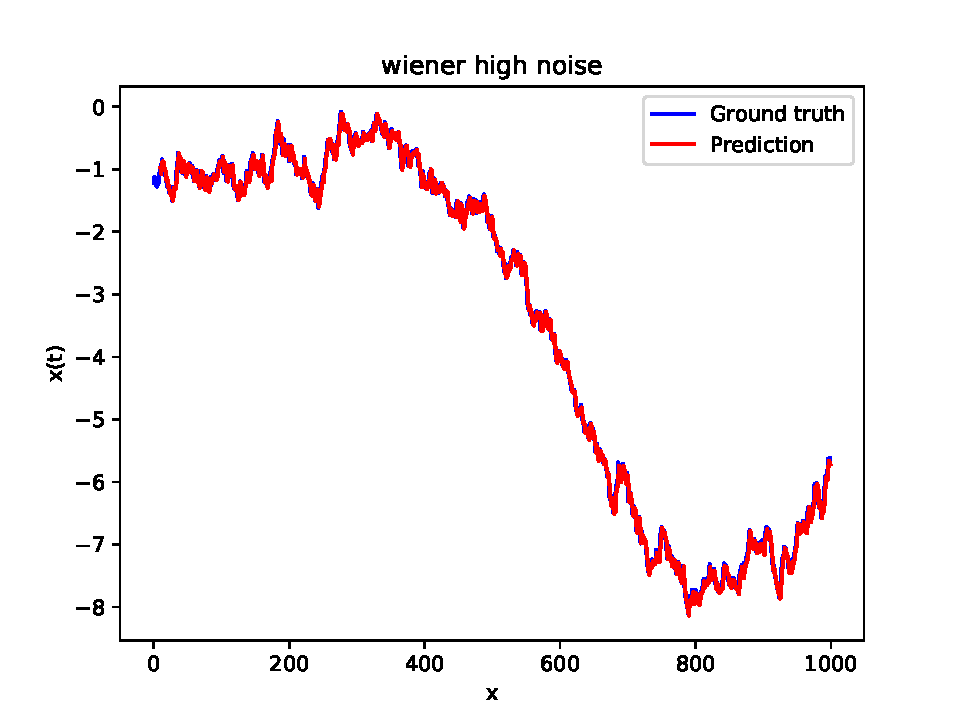
\includegraphics[width=0.45\textwidth]{figures/wiener_high_noise.pdf}
    \caption{Demonstration of grid search results. The low noise has a
    standard deviation of $\sigma =0.01$ and the high noise uses $\sigma=0.1$,
    independent of the type of noise.}
    \label{fig:sineresult}
\end{figure}

\begin{figure}
    \centering
    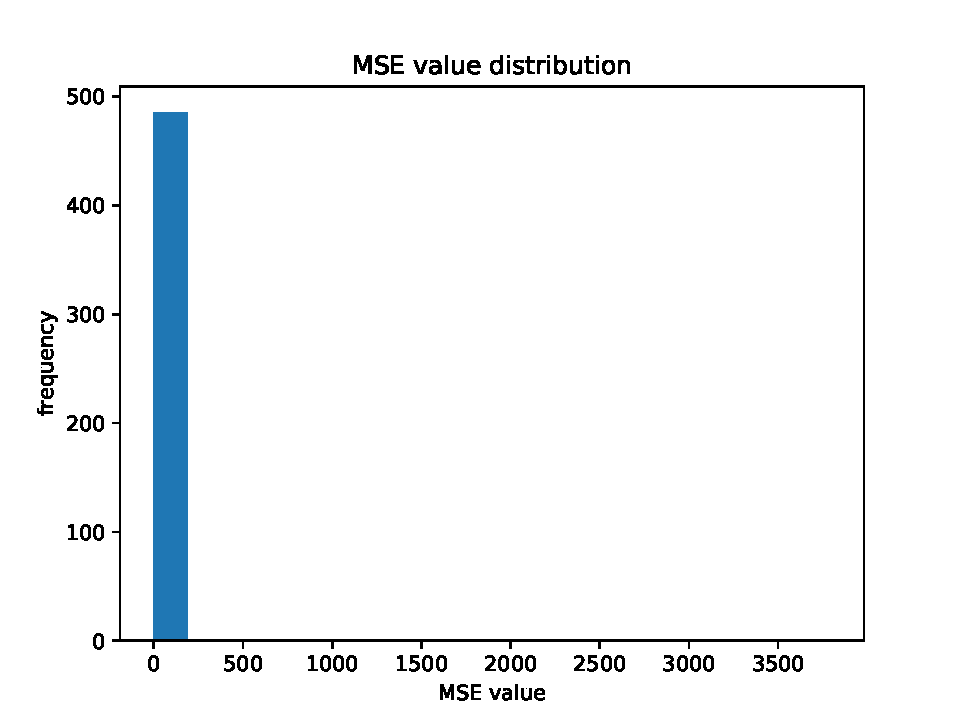
\includegraphics[width=0.6\textwidth]{figures/histogram.pdf}
    \caption{Demonstration of grid search results. A few networks with high
    test error have to be considered during the evaluation to get more 
    robust interpretations. The majority of trained networks yield smaller
    test error values.}
    \label{fig:histogram}
\end{figure}

\begin{table}
    \centering
    \begin{tabular}{l|c|c|c}
        Architecture & Noisefree data & $i.i.d.$ noise & memorizing noise \\
        \hline
        MLP          & 0.0021         & 0.0249         & 0.0174           \\
        LSTM         & 0.0021         & 0.0127         & 0.5554           \\
        CNN          & 0.0021         & 0.0136         & 0.0234           \\
    \end{tabular}
    \caption{Validation loss of different neural network architectures for
        time series prediction on the sinus function stated
        in RMSE.}
    \label{tab:noise_finals}
\end{table}

\subsection{Mackey-Glass time series forecasting}

In order to model diseases related to dynamic respiratory and hematopoietic
diseases, Mackey \textit{et al.} proposed the Mackey-Glass equations, a kind of
first-order nonlinear differential delay equations to model
the number of white blood cells over time \cite{mackey1977}. The solutions to
these equations given in Equation~\ref{equ:mackey}
exhibit chaotic behavior under certain conditions \cite{farmer1982}. For fixed
parameters $a = 0.2$, $b=0.1$ and $c=10$ this system has a stable fixed point
attractor for $\tau < 4.53$. With increasing delay time, the system gets less
stable. For delay times of $4.53 < \tau < 13.3$ there is a limit cycle attractor
whose period raises for $13.3 \leq \tau \leq 16.8$. For delay time
$\tau > 16.8$ the system shows chaotic behavior.

\begin{equation}
    \frac{dx}{dt} = \frac{a \cdot x(t - \tau)}{1 + x(t - \tau)^c} - b \cdot x(t)
    \label{equ:mackey}
\end{equation}

By using the Euler method to discretize the Mackey-Glass time series shown in 
Equation~\ref{equ:mackey_euler}, we can
see that the chaotic behavior gets stronger for increasing $\tau > 16.8$. In
Figure~\ref{fig:mackey_chaos}, we simulate the solution of the Mackey-Glass
time series for slightly different initial conditions. It is clearly visible
that for $\tau = 17$, the time series diverges slower than for $\tau = 25$. In 
the phase plot in that figure we can see that the trajectory of the time delay 
$\tau = 17$ looks still similar to the non-chaotic trajectory of the time delay
$\tau = 15$. But for $\tau=25$, the chaos is so strong such that no similarity 
to the non-chaotic trajectories can be recognized.

The first approach to predict the short-time behavior of chaotic time series
was done by Farmer \textit{et al.} who proposed a \texttt{local approximation}
technique \cite{farmer1987}. After improval of predictions using support vector
machines by Müller \textit{et al.} \cite{muller1997}, the focus in research
shifted towards artifical neural networks which enabled even better predictions.
Two of the latest developments are the usage of Wavelet Networks
\cite{alexandridis2013} and particle swarm optimization \cite{lopez2016}.

\begin{equation}
    x(t+1) = x(t) + \frac{\beta x(t - \tau)}{1 + x^{n}(t - \tau)} - \gamma x(t)
    \label{equ:mackey_euler}
\end{equation}

\begin{figure}
    \centering
    \begin{subfigure}{.51\textwidth}
        \centering
        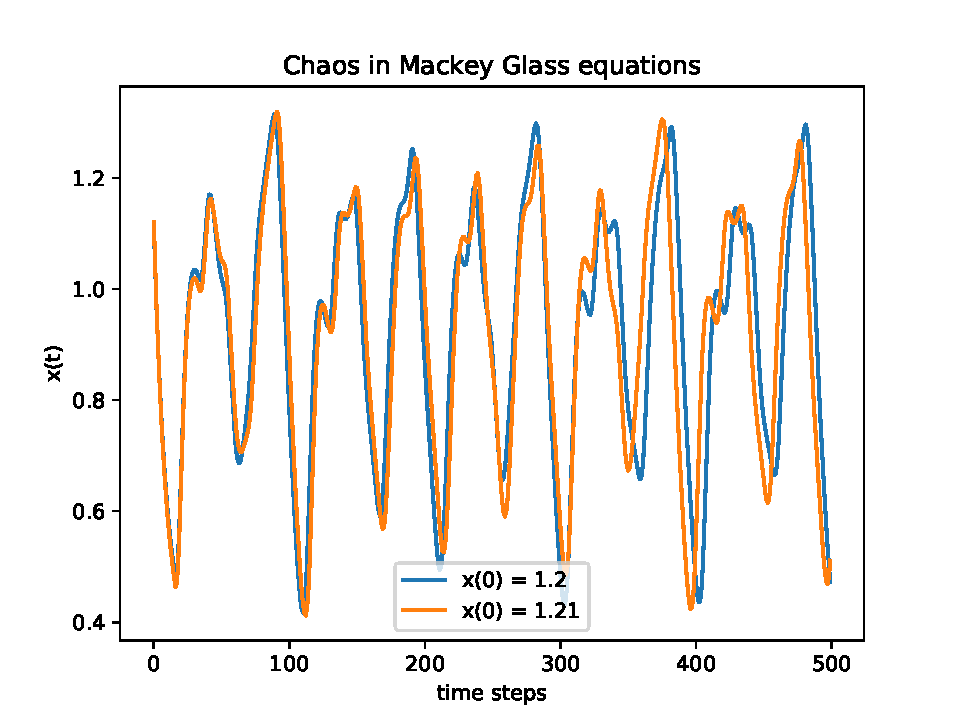
\includegraphics[width=\textwidth]{figures/mg_chaos_17.pdf}
        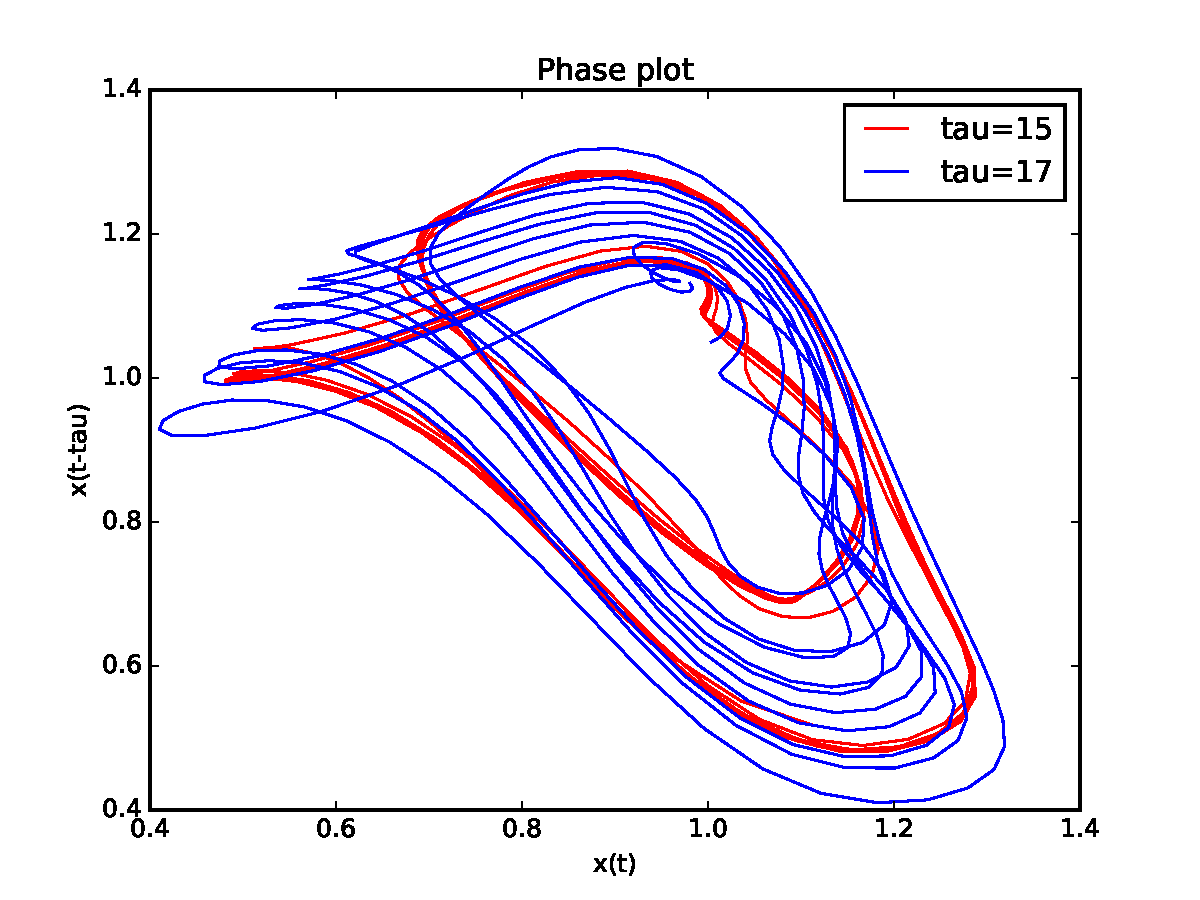
\includegraphics[width=\textwidth]{figures/17.pdf}
    \end{subfigure}
    \hspace{-6mm}
    \begin{subfigure}{.51\textwidth}
        \centering
        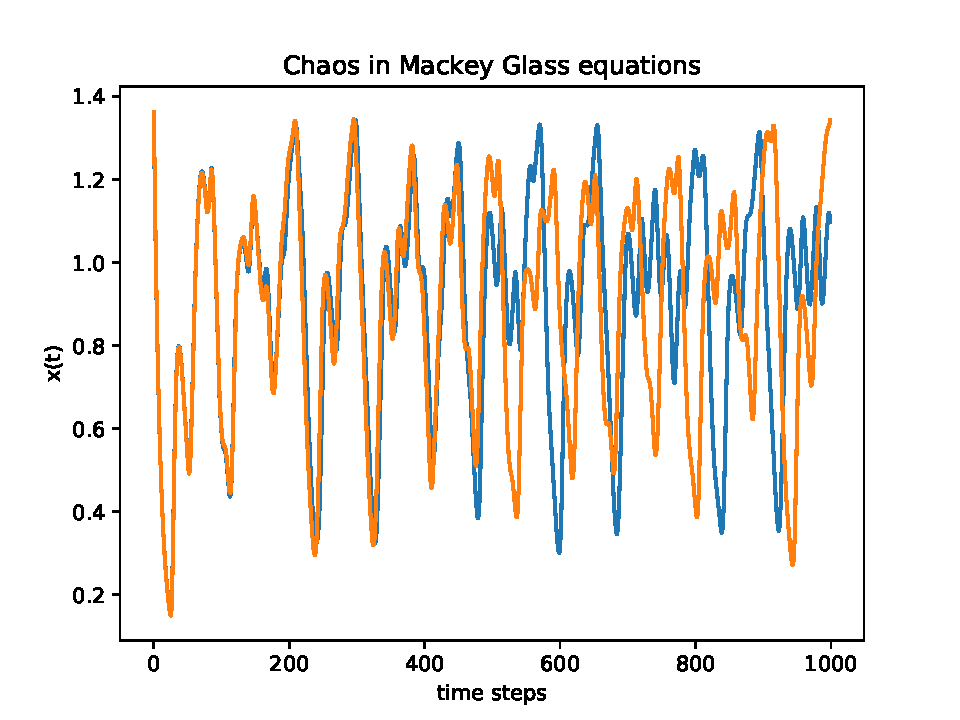
\includegraphics[width=\textwidth]{figures/mg_chaos_25.pdf}
        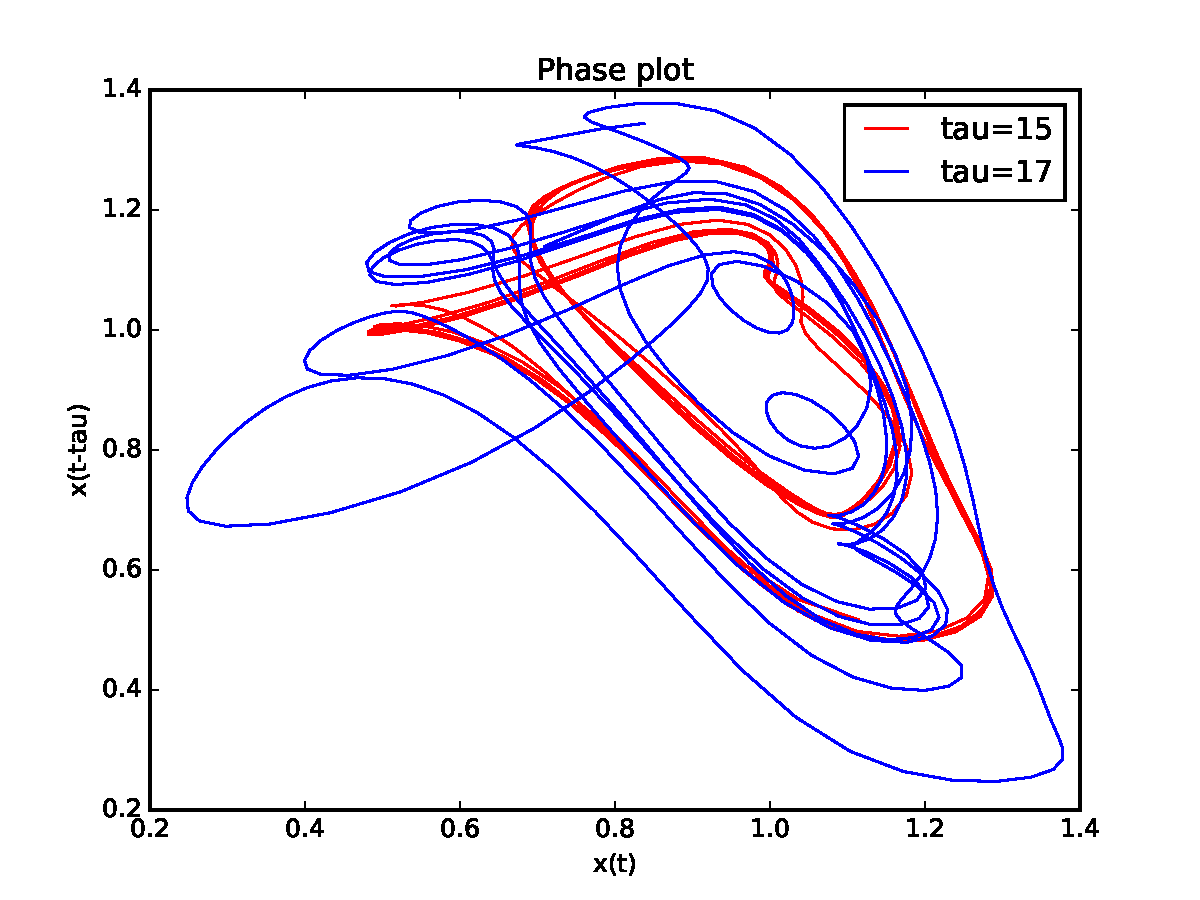
\includegraphics[width=\textwidth]{figures/25.pdf}
    \end{subfigure}
    \caption{Influence of time delay parameter $\tau$ on the chaotic behavior of
        the Mackey-Glass equation. The top left side of the figure
        uses $\tau = 17$, the right side $\tau = 25$. The phase plot for 
        $\tau=17$ shows additionally the phase plot for $\tau=15$ to visualize 
        the similarity with a time series which is not chaotic, but has 
        a limit cycle attractor instead.}
    \label{fig:mackey_chaos}
\end{figure}

In accordance with the approach used by López-Caraballo \textit{et al.}
\cite{lopez2016}, we predict $x(t+6)$ based on the information of the time
series points in $x(t)$, $x(t-6)$, $x(t-12)$, and $x(t-18)$. We investigate how
an increase in chaotic behavior impacts the prediction capability of the
different neural network architectures. The results for the \emph{LSTM}
are depicted in Figure~\ref{fig:mackey_lstm}. For this plot, a 2-layer
LSTM architecture is used, using 10 hidden nodes in the LSTM layer,
followed by a feedforward layer to sum up for the output value.
The first 500 time points of the time series are used for training, the 500
following points for validation. Additional 500 points are not used during the
training procedure at all and form the test set. For training our models, we 
train the models for 100 epochs. The learning rate of $0.01$ for the Adam 
optimizer, because it outperforms the default learning rate in this situation.

It can be seen that for non-chaotic solutions of the macke-glass time series the
model is able to predict precisely, and that for values of $\tau > 20$ the
chaotic behavior is strong enough to impact the prediction. We explain the low
error for $\tau = 21$ in the ability of the network to compensate for the amount
of chaos up to this point.

\begin{figure}
    \centering 
    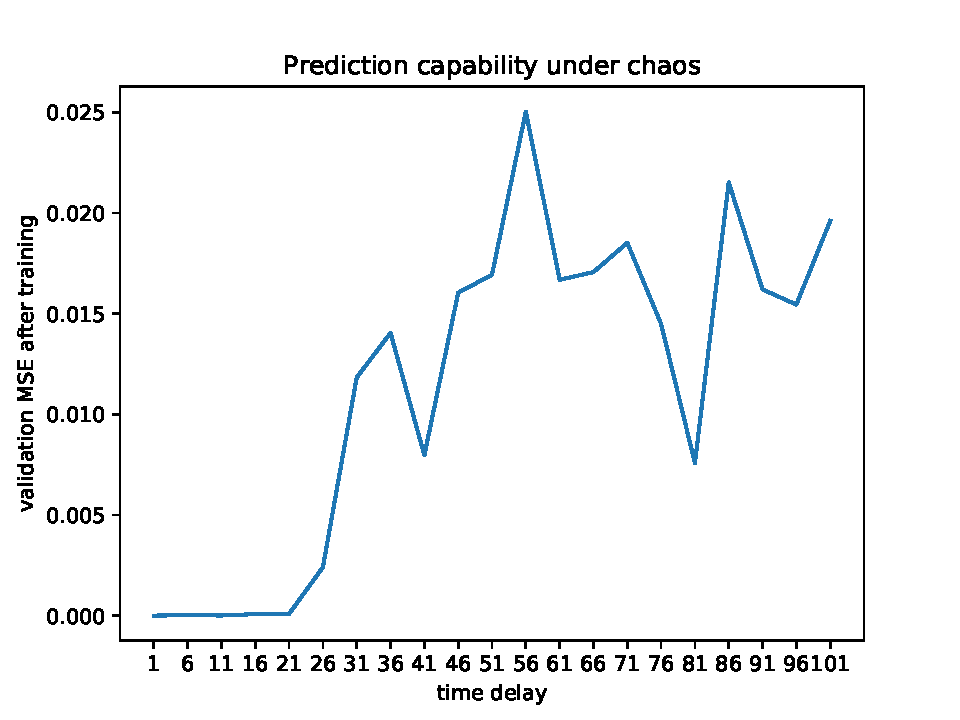
\includegraphics[width=0.6\textwidth]{figures/mackey_glass_lstm_fast.pdf}
    \caption{Validation error of the \emph{LSTM} network for different
        time delay values $\tau$ of the Mackey-Glass equation. The error increases
        strongly for values of $\tau > 20$, indicating a strong chaotic behavior
        from this point.}
    \label{fig:mackey_lstm}
\end{figure}

In the next step, we compare our \emph{MLP}, our \emph{LSTM} and our \emph{CNN}
architectures with the results stated by López-Caraballo \textit{et al.}
\cite{lopez2016} in Table~\ref{tab:mackey_results}. We
compare our results with a linear model, a cascade correlation neural network
and a radial basis function (\emph{RBF})
neural network additional to their approach to
combine an artificial neural network (\emph{ANN}) with particle swarm
optimization (\emph{PSO}). By
using the \emph{ReLU} (Rectified Linear Unit) activation function and two
hidden layers with 32 and 16 nodes, respectively, we outperform the
backpropagation network reported by López-Caraballo \textit{et al}.
From our considered models, the \emph{CNN} achieves the lowest RMSE value and
allows for accurate prediction, both for validation and for test data as seen
in Figure~\ref{fig:mackey_pred}. This \emph{CNN} uses three convolutional layers
with 1D convolutions, kernel size of 3, "same" padding and 8
filters each. A classical
feedforward layer without activation function is used to extract the output
value for the time series prediction. We avoid overfitting successfully, since
the test data of the chaotic time series was never presented to the neural
network, but is predicted accurately.

The \emph{LSTM} employs 10 LSTM nodes, followed by a feedforward layer to sum up
the results. A variety of other layer configurations has been applied
on the problem,
but all consistently perform worse than the other neural network architectures.
We assume that the chaotic behavior of the time series confuses the \emph{LSTM}
which is trying to account for temporal dependencies between the time series
points.

\begin{figure}
    \centering
    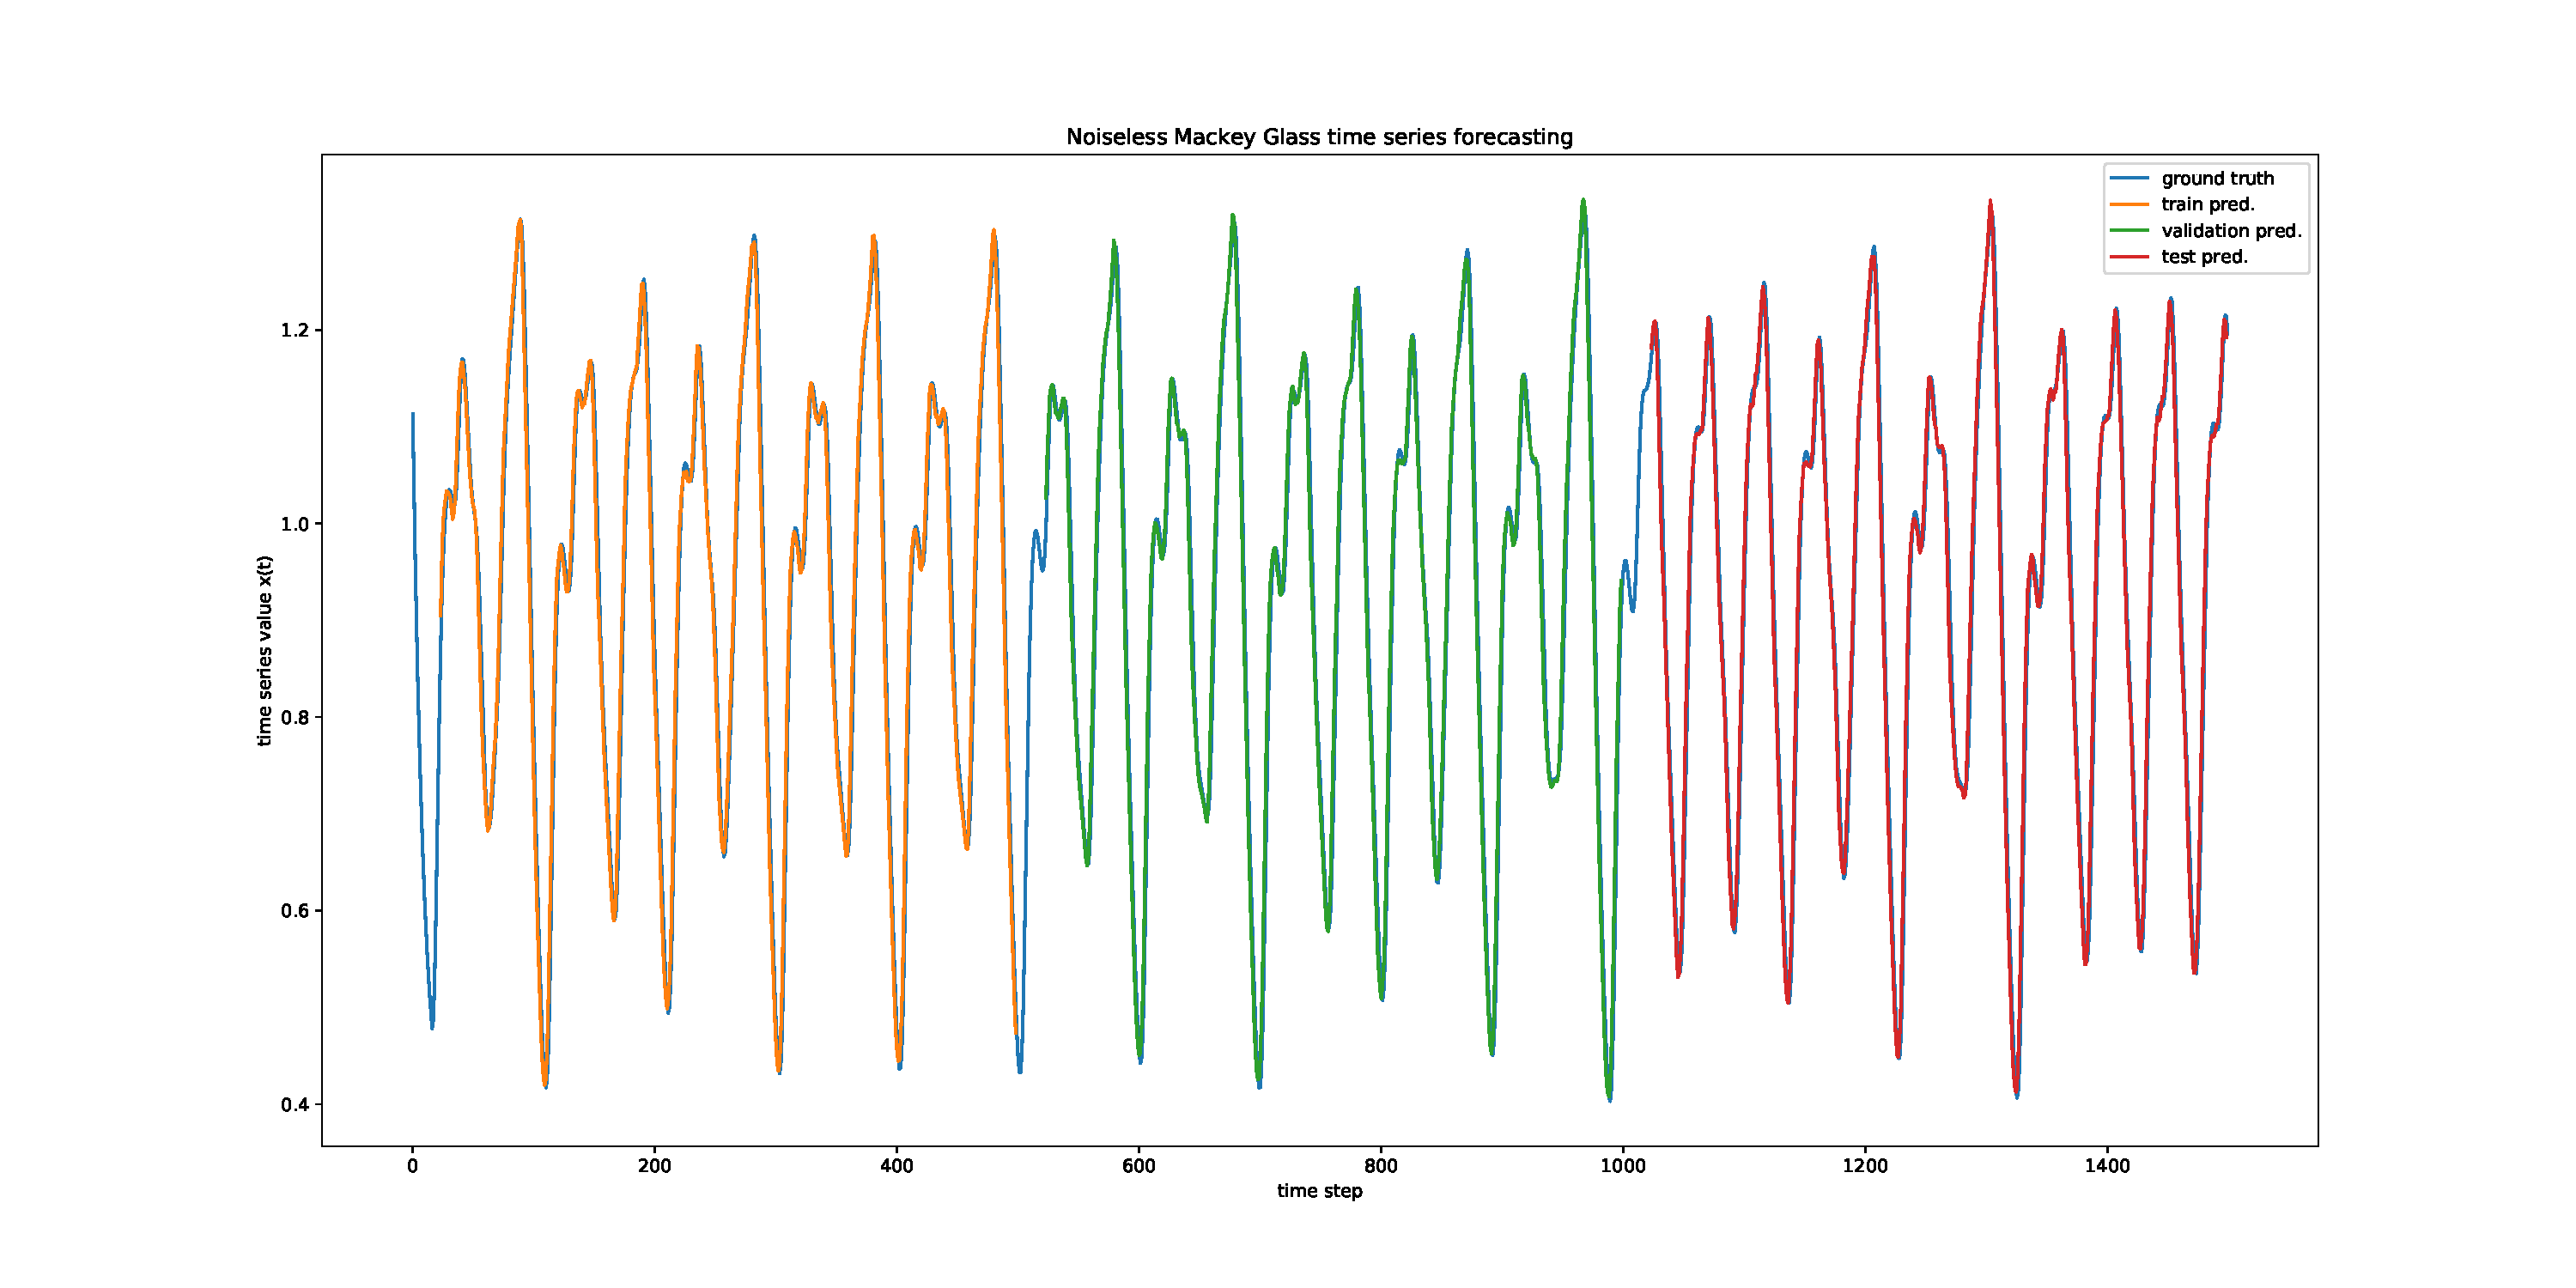
\includegraphics[width=\textwidth]{figures/mg_pred_cnn.pdf}
    \caption{The prediction of the noisefree Mackey-Glass time series using a
        \emph{CNN} with $3$ hidden layers.
        The precise predictions for training, validation and testing
        points show the accurate approximation of the chaotic time series.}
    \label{fig:mackey_pred}
\end{figure}

\begin{table}
    \centering
    \begin{tabular}{c|c}
        Method                         & $RMSE_{x(t+6)}$                          \\
        \hline
        Linear model                   & 0.5503                                   \\
        Cascade correclation NN        & 0.0624                                   \\
        \textit{proposed LSTM}         & 0.0131                                   \\
        \textit{proposed MLP}          & 0.0125 (vs. 0.0262 \cite{lopez2016}) \\
        RBFNN                          & 0.0114                                   \\
        \textit{proposed CNN}          & 0.0075                                   \\
        ANN + PSO \cite{lopez2016} & 0.0053                                   \\
    \end{tabular}
    \caption{Mackey-Glass time series forecasting results using different neural
        network architectures.}
    \label{tab:mackey_results}
\end{table}

Now we apply noise on the Mackey-Glass time series to account for the imperfect
data typical for biological measurements. The results for these
experiments are stated in Table~\ref{tab:mackey_noise}. We see that an increased
standard deviation of the added noise increases the test error, measured in
RMSE. This applies to all neural network architectures.

We interpret the results of Table~\ref{tab:mackey_noise}
as the neural networks are capable of dealing with a certain
amount of noise. For example the \emph{CNN} has
approximately 9 times higher error rate when increasing the standard 
deviation of the Wiener process from $0.01$ to $0.1$.

But more interestingly,
the negative effect of the noise is stronger if the noise is memorizing, i.e. if
the effect of the noise in time step $t$ impacts the time series in time step
$t + 1$. We explain this with an increase in chaotic behavior induced by this
type of noise to the Mackey-Glass time series. Since chaotic time series by
definition deviate exponentially based on small variations in the initial
conditions, it seems logical that this divergence is increased by introducing
perturbations of the time series in every time step.

\begin{table}
    \centering
    \begin{tabular}{c|c|c|c}
        Architecture & noise type & $\sigma$ & RMSE   \\
        \hline
        CNN          & iid        & 0.01     & 0.0196 \\
        CNN          & iid        & 0.1      & 0.0806 \\
        CNN          & wiener     & 0.01     & 0.0242 \\
        CNN          & wiener     & 0.1      & 0.2172 \\
        MLP          & iid        & 0.01     & 0.0249 \\
        MLP          & iid        & 0.1      & 0.0949 \\
        MLP          & wiener     & 0.01     & 0.0348 \\
        MLP          & wiener     & 0.1      & 0.2162 \\
        LSTM         & iid        & 0.01     & 0.0432 \\
        LSTM         & iid        & 0.1      & 0.0862 \\
        LSTM         & wiener     & 0.01     & 0.0347 \\
        LSTM         & wiener     & 0.1      & 0.2044 \\
    \end{tabular}
    \caption{Results of the Mackey-Glass time series forecasting using different
        types of neural networks, noise levels and types.}
    \label{tab:mackey_noise}
\end{table}

\subsection{Biological oscillator time series forecasting}

The next section deals with time series generation of biological oscillators,
as described by Novak \textit{et al} \cite{novak2008}. For different aspects of
cell physiology, e.g. the DNA synthesis, this kind of oscillators can be
observed. Novak \textit{et al.} show that oscillations in simple ODEs can be
produced by incorporating an explicit time delay \cite{novak2008}, similar to
the Mackey-Glass equations \cite{mackey1977}.

Recently, Strömstedt \textit{et al.} analyzed the capability of neural network
architectures to model stochastic time series \cite{stroemstedt2018} at the
example of time series produced according to the characteristics of Novak
\textit{et al} \cite{novak2008}. In this section, we reproduce their results for
the LSTM architecture and state fundamental limits for neural networks to
approximate stochastic time series.

The \texttt{gillespy} framework is used to 
model a stochastic reaction system with 2 states as defined 
in Equation~\ref{equ:oscillator}.
One protein $X$ is produced more the less of the other protein $Y$
exists. $X$ and $Y$ are both continuously reduced but $Y$ gets reduced stronger
for smaller values of $Y$ in a non-linear way. A set of 6 parameters
($k_{dx}, k_t, k_{dy}, a_0, a_1, a_2)$
is used to parametrize the system.

\begin{align}
    \frac{dX}{dt} = & \frac{1}{1+Y^2} - k_{dx} \cdot X                                           \\
    \frac{dY}{dt} = & k_t \cdot X - k_{dy} \cdot Y - \frac{Y}{a_0 + a_1 \cdot Y + a_2 \cdot Y^2}
    \label{equ:oscillator}
\end{align}

The motivation for using neural networks to generate time series is the
computational expensiveness of analytical solutions like the Gillespie
algorithm \cite{gillespie1977}. The runtime of an experiment on our hardware
(see Table~\ref{tab:hardware} for details)
takes more than 6 seconds runtime to simulate this biological oscillator with
two states for 100 time steps (yielding only one trajectory of the stochastic
system). This makes grid search approaches on the large number
of parameter
combinations intractable. Using the 2-layer LSTM approach, predictions for
short time series can be done in less than $0.2$ seconds on our hardware.

The goal here is to train a LSTM based
model to convert a set of input parameters into a time series. The first
LSTM layer
takes 7 input values and transforms them into $n$ sequences of 7 values, with
$n$ being the desired length of the output sequence. The second LSTM layer
takes this intermediate result and converts it to a sequence of length $n$.

The analysis of the resulting time series as depicted in
Figure~\ref{fig:nn_limitation} shows the general limitation of using a
deterministic neural network for predicting a stochastic time series. For one
possible of parameters for the biological oscillator, the analytical solution
was computed under $100$ (stochastic) trajectories. After that, the network was
trained to predict the time series based on the (unchanged) parameters. We see
that the short-term predictions are accurate and have the same magnitude as the
ground truth signal -- but the more time steps are simulated, the larger is the
difference between the ground truth trajectories due to stochasticity. In other
words, the neural network predicts the mean of the signals and the amplitude
decreases due to the increasing variance of the signal over time.
It should be noted that the trends in the time series are still
recognized, just with a smaller amplitude.

\begin{table}
    \centering
    \begin{tabular}{cc}
        Processor & Intel(R) Core i5-7200U CPU @ 2.50GHz \\
        RAM       & 7859 MB                              \\
    \end{tabular}
    \caption{Hardware configuration used in experiments.}
    \label{tab:hardware}
\end{table}

\begin{figure}
    \centering
    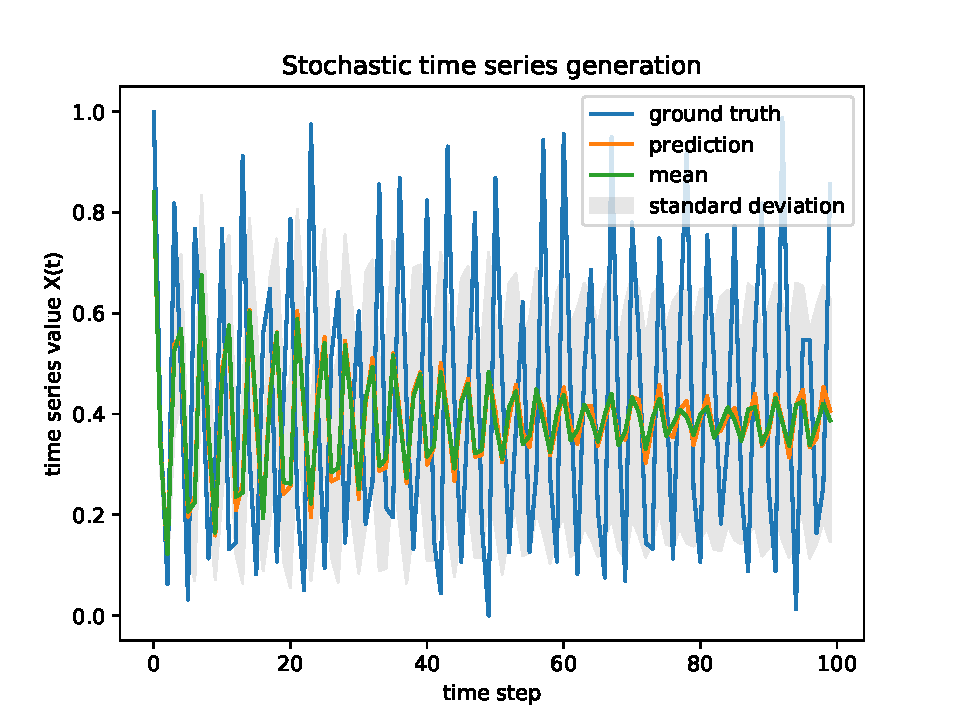
\includegraphics[width=\textwidth]{figures/nn_limitation.pdf}
    \caption{Prediction of stochastic time series using deterministic
        \textbf{LSTM} network. Sampled ground truth data are unseen for the network.
        Mean computed on all stochastic trajectories.}
    \label{fig:nn_limitation}
\end{figure}
